\documentclass[a4paper,10pt]{article}

% packages
\usepackage[utf8]{inputenc} % allows usage of spanish special characters
\usepackage[spanish,english]{babel} % english dictionary for proper hyphenation
\usepackage{amsmath} % math expressions
\usepackage{upgreek} % upright greek letters for math
\usepackage{txfonts} % nice fonts 
\usepackage{authblk} % author affiliations
\usepackage{graphicx} % images
\usepackage{float} % image positioning
\usepackage{multirow} % allows merging cells in tables
\usepackage{makecell} % more table customization
\usepackage{mathtools} % nice matrices
\usepackage{units} % nice fractions
\usepackage{rotating} % rotated text
\usepackage{caption} % customization of figure/table captions
\usepackage{subcaption} % collages of multiple images
\usepackage{hyperref} % hyperlinks
\usepackage{nameref} % cross-references between draft and supplementary material
\usepackage{zref-xr,zref-user} % more cross-references formatting
\usepackage[square,numbers,sort&compress]{natbib}
\usepackage[table,xcdraw]{xcolor} % text and table background colors
\usepackage[margin=3cm]{geometry} % margins
\usepackage{lineno} % line numbers

\usepackage{pdflscape} %% Landscape
\usepackage{dcolumn}
\usepackage{booktabs}
\usepackage{savesym}
\savesymbol{iint}
\restoresymbol{TXF}{iint}
%% \usepackage{pdfpages} %% to include a pdf file

% customization
\setcounter{Maxaffil}{0} % affiliations
\renewcommand\Affilfont{\itshape\small} % style of affiliations text
\makeatletter\renewcommand{\@biblabel}[1]{#1.}\makeatother % change [number] for number. in reference list
\addto{\captionsenglish}{\renewcommand{\bibname}{References}}
\newcommand{\idea}[1]{\textcolor{red}{#1}}
\newcommand{\mr}{\textcolor{red}{\textbf{[missing ref(s)]}}}
\newcommand{\Burl}[1]{\url{#1}}
\zxrsetup{toltxlabel} % cross references: draft & suppl mat
\zexternaldocument*[M-]{draft}
\hypersetup{
  colorlinks = true,
  citecolor=  black,
  linkcolor = {blue},
  filecolor = cyan % controls color of external ref, if used
}
\captionsetup[figure]{font=small, labelfont={bf}, labelformat={default},
   labelsep=period, name={Figure}} % custom figure captions
\captionsetup[table]{font=small, labelfont={bf}, labelformat={default},
   labelsep=period, name={Table}} % custom table captions
\hypersetup{citecolor={blue}}
\definecolor{lightgray}{gray}{0.9}

% title, authors, affiliations
\title{Provisional Title}
\author[1,2,3]{Authors}
\author[1,2,$\dagger$]{Álvaro Sánchez}
\affil[1]{Department of Ecology \& Evolutionary Biology,
Yale University, New Haven, CT, USA}
\affil[2]{Microbial Sciences Institute,
Yale University, New Haven, CT, USA}
\affil[3]{Other affiliations...}
\affil[$\dagger$]{To whom correspondence should be addressed: \normalfont alvaro.sanchez@yale.edu}
\date{}



  
\begin{document}

\linenumbers

\maketitle

\begin{abstract}
  
The abstract goes here.
  
\end{abstract}

\section*{Introduction}\label{intro}

This is an example cite \cite{Vetrovsky2013,nloptr}

\section*{Results \& Discussion}\label{results-discussion}

This is how you refer to the \nameref{intro}.

\clearpage

\section*{Methods}\label{methods}

\subsection*{Stabilization of environmental communities in simple synthetic environments}
\label{methods:community-assembly}

Communities were stabilized \textit{ex situ} as described in \cite{Goldford2018}.
In short, environmental samples (soil, leaves...) within one meter radius in eight different
geographical locations were collected with sterile
tweezers or spatulas into 50mL sterile tubes (Fig. \mr).
One gram of each sample was allowed to
sit at room temperature in 10mL of phosphate buffered saline (1$\times$PBS) containing
200$\upmu$g/mL cycloheximide to suppress eukaryotic growth.
After 48h, samples were mixed 1:1 with 80\% glycerol and kept frozen at $-80^\circ$C.
Starting microbial communities were prepared by scrapping the frozen stocks into
$200\upmu$L of 1$\times$PBS and adding a volume of $4\upmu$L to $500\upmu$L
of synthetic minimal media (1$\times$M9) supplemented with $200\upmu$g/mL cycloheximide
and 0.07 C-mol/L glutamine or sodium citrate as the carbon source in 96 deep-well plates
(1.2mL; VWR).
Cultures were then incubated still at $30^\circ$C to allow for re-growth.
After 48h, samples were fully homogenized and biomass increase was followed by measuring
the optical density (620nm) of $100\upmu$L of the cultures in a Multiskan FC plate reader
(Thermo Scientific).
Communities were stabilized \cite{Goldford2018} by passaging $4\upmu$L of the cultures into
$500\upmu$L of fresh media (1$\times$M9 with the carbon source)  every 48h for a total of
12 transfers at a dilution factor of 1:100,
roughly equivalent to 80 generations per culture (Fig. \mr).
Cycloheximide was not added to the media after the first two transfers.

\subsection*{Isolation of dominant species}\label{methods:dominants}

For each community, the most abundant colony morphotype at the end of the ninth transfer
was selected, resuspended in $100\upmu$L 1$\times$PBS and serially diluted (1:10).
Next, $20\upmu$L of the cells diluted to $10^{-6}$ were plated in the corresponding synthetic
minimal media and allowed to regrow at $30^\circ$C for 48h. Dominants were then inoculated
into $500\upmu$L of fresh media and incubated still at $30^\circ$C for 48h.
After this period, the communities stabilized for eleven transfers and the isolated dominants
were ready for the competition experiments (Fig \mr) at the onset of the twelfth transfer.

\subsection*{Dominant-dominant and community-community competitions}
\label{methods:competitions}

All possible pairwise dominant-dominant and community-community
competition experiments
were performed by mixing equal volumes ($4\upmu$L) of each of the eight
communities or eight dominants at the onset of the twelfth transfer.
Competitions were set up in their native media,
i.e. in $500\upmu$L of 1$\times$M9 supplemented with 0.07 C-mol/L of
either glutamine or citrate in 96 deep-well plates.
Plates were incubated at $30^\circ$C for 48h.
Pairwise competitions were further propagated for seven serial transfers
(roughly 42 generations; Fig. \mr) by transferring $8\upmu$L of
each culture to fresh media ($500\upmu$L).

\subsection*{Determination of community composition by 16S sequencing}
\label{methods:sequencing}

The sequencing protocol was identical to that described in \cite{Goldford2018}.
Community samples were collected by spinning down at 3500rpm for 25min
in a bench-top centrifuge at room temperature;
cell pellets were stored at $-80^\circ$C before processing.
To maximize Gram-positive bacteria cell wall lysis,
the cell pellets were re-suspended and incubated at $37^\circ$C for 30min
in enzymatic lysis buffer (20mM Tris-HCl, 2mM sodium EDTA, 1.2\% Triton X-100)
and 20mg/mL of lysozyme from chicken egg white (Sigma-Aldrich).
After cell lysis, the DNA extraction and purification was performed using the
DNeasy 96 protocol for animal tissues (Qiagen).
The clean DNA in $100\upmu$L elution buffer of 10mM Tris-HCl, 0.5mM EDTA
at pH 9.0 was quantified using Quan-iT PicoGreen dsDNA Assay Kit
(Molecular Probes, Inc.)
and normalized to 5ng/$\upmu$L in nuclease-free water (Qiagen)
for subsequent 16S rRNA illumina sequencing.
16S rRNA amplicon library preparation was performed following a dual-index
paired-end approach \cite{Kozich2013}.
Briefly, PCR amplicon libraries of V4 regions of the 16S rRNA were prepared 
sing dual-index primers (F515/R805), then pooled and sequenced
using the Illumina MiSeq chemistry and platform.
Each sample went through a 30-cycle PCR in duplicate of $20\upmu$L
reaction volumes using 5ng of DNA each, dual index primers, and AccuPrime Pfx SuperMix (Invitrogen).
The thermocycling procedure includes a 2min initial denaturation step at
$95^\circ$C, and 30 cycles of the following PCR scheme:
(a) 20-second denaturation at $95^\circ$C,
(b) 15-second annealing at $55^\circ$C,
and (c) 5-minute extension at $72^\circ$C.
The duplicate PCR products of each sample were pooled, purified, and normalized
using SequalPrep PCR cleanup and normalization kit (Invitrogen).
Barcoded amplicon libraries were then pooled and sequenced using
Illumina Miseq v2 reagent kit, which generated 2$\times$250bp paired-end reads
at the Yale Center for Genome Analysis (YCGA).
The sequencing reads were demultiplexed on QIIME 1.9.0 \cite{Caporaso2010}.
The barcodes, indexes, and primers were removed from raw reads,
producing FASTQ files with both the forward and reverse reads for each sample,
ready for DADA2 analysis \cite{Callahan2017}.
DADA2 version 1.1.6 was used to infer unique biological exact sequence variants
(ESVs) for each sample
and na{\"i}ve Bayes was used to assign taxonomy using the SILVA version 123
database \cite{Wang2007,Quast2013}.

\subsection*{Metrics of community distance}
\label{methods:metrics}

Beta-diversity indexes between the invasive and coalesced communities
or the resident and coalesced communities were computed using various
similarity metrics. For two arbitrary communities with
ESV abundances represented by the vectors
$\mathbf{x} = \left( x_1, x_2, \cdots, x_N \right)$
and
$\mathbf{y} = \left( y_1, y_2, \cdots, y_N \right)$
(where $x_i$ and $y_i$ represent the relative abundance of the $i$th ESV in
each community respectively and $N$ is the total number of ESVs), the Bray-Curtis
similarity $\mathrm{BC} \left( \mathbf{x}, \mathbf{y} \right)$ is calculated as
\cite{Bray1957}

\begin{equation}
\mathrm{BC} \left( \mathbf{x}, \mathbf{y} \right) = 
\sum_i \mathrm{min} \left( x_i , y_i \right)
\label{eq:bray-curtis}
\end{equation}
%
The Jensen-Shannon similarity
$\mathrm{JS} \left( \mathbf{x}, \mathbf{y} \right)$
is defined as one minus the Jensen-Shannon distance (which is, in turn,
the square root of the Jensen-Shannon divergence \cite{Lin1991})

\begin{equation}
\mathrm{JS} \left( \mathbf{x}, \mathbf{y} \right) = 
1 - \sqrt{\frac{1}{2}\mathrm{KL} \left( \mathbf{x}, \mathbf{m} \right) +
\frac{1}{2}\mathrm{KL} \left( \mathbf{y}, \mathbf{m} \right)}
\label{eq:jensen-shannon}
\end{equation}
%
where $\mathbf{m} = \left( \mathbf{x} + \mathbf{y} \right)/2$ and KL denotes the
Kullback-Leibler divergence \cite{Kullback1951}

\begin{equation}
\mathrm{KL} \left( \mathbf{x}, \mathbf{y} \right) = 
\sum_i x_i \; \mathrm{log_2} \left( \frac{x_i}{y_i} \right)
\label{eq:kullback-leibler}
\end{equation}
%
The Jaccard similarity is given by
$\mathrm{J} \left( \mathbf{x}, \mathbf{y} \right)$ \cite{Jaccard1912}

\begin{equation}
\mathrm{J} \left( \mathbf{x}, \mathbf{y} \right) = 
\frac{\left|\; \mathbf{x} \cap \mathbf{y} \;\right|}
{\left|\; \mathbf{x} \cup \mathbf{y} \;\right|}
\label{eq:jaccard}
\end{equation}
%
For all the metrics above, we quantify the relative similarity between the invasive
and the coalesced communities using relative metrics (Q):

\begin{equation}
\mathrm{Q} \left( \mathbf{x}_\mathrm{I},
\mathbf{x}_\mathrm{R},
\mathbf{x}_\mathrm{C} \right) = 
\frac{\mathrm{F} \left( \mathbf{x}_\mathrm{I},\mathbf{x}_\mathrm{C}\right)}
{\mathrm{F} \left( \mathbf{x}_\mathrm{I},\mathbf{x}_\mathrm{C}\right)
+
\mathrm{F} \left( \mathbf{x}_\mathrm{R},\mathbf{x}_\mathrm{C}\right)}
\label{eq:q}
\end{equation}
%
where the subindices I, R and C correspond to the invasive, resident and coalesced
communities respectively, and F represents one of BC (Bray-Curtis similarity), JS
(Jensen-Shannon similarity) or J (Jaccard similarity) defined in equations
\ref{eq:bray-curtis} to \ref{eq:jaccard}.

Additionally, we quantify coalescence outcomes by examining the fraction of the endemic
cohort of the invasive community that persists in the coalesced one. We denote this
metric as
$\mathrm{E} \left( \mathbf{x}_\mathrm{I},
\mathbf{x}_\mathrm{R},
\mathbf{x}_\mathrm{C} \right)$.


\begin{equation}
\mathrm{E} \left( \mathbf{x}_\mathrm{I},
\mathbf{x}_\mathrm{R},
\mathbf{x}_\mathrm{C} \right) = 
\left.
\sum_i
f \left( x_{\mathrm{I}i}, x_{\mathrm{R}i}, x_{\mathrm{C}i} \right)
\;
\middle/
\;
\sum_i
g \left( x_{\mathrm{I}i}, x_{\mathrm{R}i} \right)
\right.
\label{eq:endemic}
\end{equation}
%
where we have defined

\begin{equation}
\begin{split}
f \left( x_{\mathrm{I}i}, x_{\mathrm{R}i}, x_{\mathrm{C}i} \right) & =
\begin{cases}
    1 & \text{if } x_{\mathrm{I}i} > 0 \text{ and }
                   x_{\mathrm{R}i} = 0 \text{ and }
                   x_{\mathrm{C}i} > 0 \\
    0 & \text{otherwise}
\end{cases} \\
g \left( x_{\mathrm{I}i}, x_{\mathrm{R}i} \right) & =
\begin{cases}
    1 & \text{if } x_{\mathrm{I}i} > 0 \text{ and }
                   x_{\mathrm{R}i} = 0 \\
    0 & \text{otherwise}
\end{cases}
\end{split}
\label{eq:endemic-f}
\end{equation}

\subsection*{Simulations}\label{methods:sim}

We used the Community Simulator package \cite{Marsland2020} and included new
features for our simulations. In the package,
species are characterized by their resource uptake rates ($c_{i\alpha}$ for
species $i$ and resource $\alpha$), and they all
share a common metabolic matrix $\mathbf{D}$.
The element $D_{\alpha\beta}$
of this matrix represents the fraction of energy in the form of resource $\alpha$
secreted when resource $\beta$ is consumed.
Here we implemented a new operation mode
in which species can secrete different metabolites (and/or
in different abundances) when consuming a same resource. Experimental observations
support the idea of distinct species producing different sets of byproducts when
growing in the same primary resource \mr. We call $D_{i\alpha\beta}$ to the
fraction of energy in the form of resource $\alpha$ secreted \textit{by species
i} when consuming resource $\beta$ ---note that now $D_{i\alpha\beta}$ need not be
equal to $D_{j\alpha\beta}$ if $i \neq j$, unlike in the original Community
Simulator. In the package's underlying Microbial Consumer Resource Model
\cite{Goldford2018,Marsland2019}, this just means that the energy flux
$J^{\mathrm{out}}_{i\beta}$ now takes the form

\begin{equation}
J^{\mathrm{out}}_{i\beta} = \sum_\alpha D_{i\beta\alpha} l_\alpha J^{\mathrm{in}}_{i\alpha}
\label{eq:jout}
\end{equation}
%
The documentation for the Community Simulator contains detailed
descriptions of the model, parameters and package use. For the updated package with
the new functionality, see \nameref{datacode}.

For our simulations,
we first generate a library of 660 species (divided into three specialist
families of 200 members each
and a generalist family of 60 members)
and 30 resources (divided into three classes of 10 members each).
We split this library into two non-overlapping pools of 330 species each.
We randomly sample 50 species from each pool in equal ratios to seed
100 resident and
100 invasive communities respectively.
We then grow and dilute the communities serially,
replenishing the primary
resource after each dilution.
We repeat the process 20 times to ensure generational equilibrium is
achieved \cite{Goldford2018}.
We then perform the \textit{in silico} experiments by using the
generationally stable communities to seed 100 coalesced communities
that we again stabilize as described previously.
Similarly, we identify the dominant (most
abundant) species of every resident and invasive community to carry out pairwise
competition and single invasion simulations.
Most parameters are set to the defaults of the original Community Simulator
package. Table \mr shows those that are given non-default values to ensure
enough variation in the primary communities.

\section*{Data \& code availability}\label{datacode}

Experimental data and code for the analysis, as well as code for the simulations
and the updated Community Simulator package with instructions for the
new features can be found in \url{github.com/jdiazc9/coalescence}.

\section*{Acknowledgements}

The authors wish to thank Joshua Goldford, Pankaj Mehta, Wenping Cui,
Robert Marsland and all members of the Sanchez laboratory
for many helpful discussions.
We also wish to express our gratitude to the Goodman laboratory at Yale
for technical help during the early stages of this project.
The funding for this work partly results from a Scialog Program
sponsored jointly by the Research Corporation for Science Advancement and
the Gordon and Betty Moore Foundation through grants to Yale University by the
Research Corporation and the Simons Foundation.

\clearpage

% references
\clearpage
\bibliographystyle{mystyle}
%\bibliographystyle{unsrt}
\bibliography{refs}

\clearpage

\section*{Figures}\label{figs}

\begin{figure}[!h]
\centering
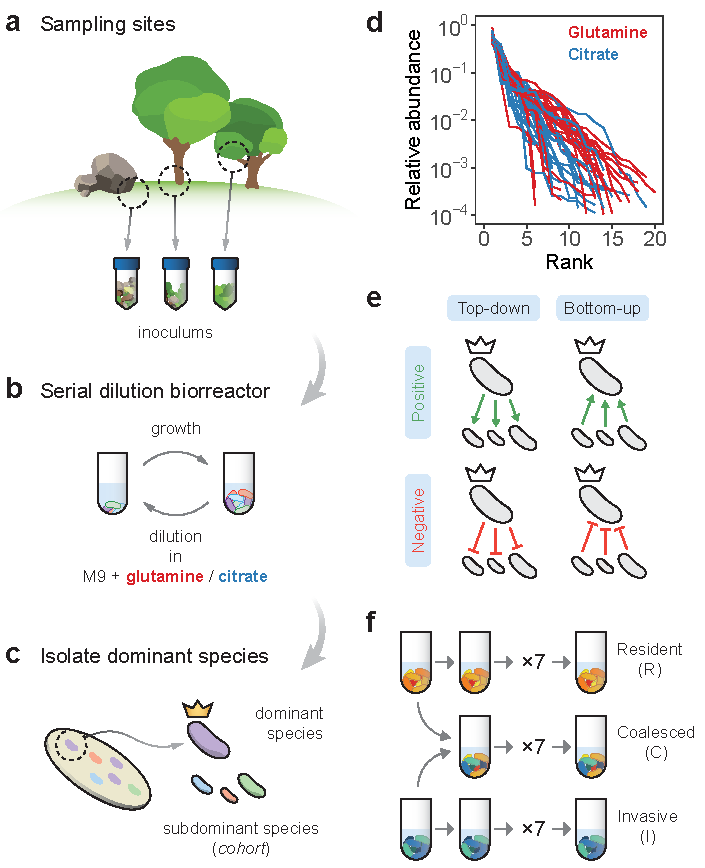
\includegraphics[width=12cm,keepaspectratio]{figs/fig1.pdf}
\caption{\textbf{Overview of the experimental protocol.}
\textbf{a.}~Environmental samples collected from eight different locations were used
to inoculate our communities.
\textbf{b.}~Communities were stabilized in serial batch culture bioreactors
\cite{Goldford2018} in minimal synthetic media with glutamine or citrate as the
only supplied carbon source.
\textbf{c.}~Communities were plated in minimal media agar plates and the most abundant
species (the ``dominants") from each community were isolated. We refer to the set of
sub-dominant species as the ``cohorts".
\textbf{d.}~Rank-frequency distributions of all eight communities stabilized in either
glutamine (red) or citrate (blue), sequenced at a depth of $10^{-4}$ reads.
Three biological replicates per community are shown.
Community compositions are skewed and long-tailed.
\textbf{e.}~Our hypothesis is that ecological co-selection can take place from the top-down,
i.e. the dominant co-selecting the cohort, or from the bottom-up, i.e. the cohort co-selecting
the dominant. Both forms of co-selection can be positive (recruitment) or negative
(antagonism).
\textbf{f.}~Illustration of the protocol of our coalescence experiments. All pairs of
communities were inoculated into fresh minimal media supplemented with the same carbon
source where communities had been previously stabilized. The coalesced (C) and original
resident (R) and invasive (I) communities were then serially diluted and allowed to grow
for seven additional transfers.}
\label{fig1}
\end{figure}

\clearpage

\end{document}




















